% !TEX TS-program = xelatex
% !BIB program = bibtex
% !TEX encoding = UTF-8 Unicode

\documentclass[
  twoside,
  openright,
  degree    = master,               % degree = master | doctor
  language  = english,              % language = chinese | english
  fontset   = template,             % fontset = default | template | system | overleaf
  watermark = false,                 % watermark = true | false
  doi       = false,                 % doi = true | false
]{ntuthesis}

% !TeX root = ./main.tex

% --------------------------------------------------
% 資訊設定(Information Configs)
% --------------------------------------------------

\ntusetup{
  university*   = {National central University},
  university    = {國立中央大學},
  college       = {理學院},
  college*      = {College of Natural Sciences},
  institute     = {物理研究所},
  institute*    = {Institute of Physics},
  title         = {國立中央大學碩博士畢業論文},
  title*        = {National Central University (NCU) \\ Thesis/Dissertation},
  author        = {劉威呈},
  author*       = {Wei-Cheng Liu},
  ID            = {108222002},
  advisor       = {周紹暐},
  advisor*      = {Dr. Shao-Wei Chou},
  date          = {2020-05-01},         % 若註解掉,則預設為當天
  oral-date     = {2020-05-01},         % 若註解掉,則預設為當天
  DOI           = {10.5566/NTU2018XXXXX},
  keywords      = {LaTeX, 中文, 論文, 模板},
  keywords*     = {LaTeX, CJK, Thesis, Template},
}

% --------------------------------------------------
% 加載套件(Include Packages)
% --------------------------------------------------
\usepackage{biblatex}
\addbibresource{back/references.bib}

%\usepackage[sort&compress]{natbib}      % 參考文獻
\usepackage{amsmath, amsthm, amssymb}   % 數學環境
\usepackage{ulem, CJKulem}              % 下劃線、雙下劃線與波浪紋效果
\usepackage{booktabs}                   % 改善表格設置
\usepackage{multirow}                   % 合併儲存格
\usepackage{diagbox}                    % 插入表格反斜線
\usepackage{array}                      % 調整表格高度
\usepackage{longtable}                  % 支援跨頁長表格
\usepackage{paralist}                   % 列表環境


\usepackage{lipsum}                     % 英文亂字
\usepackage{zhlipsum}                   % 中文亂字

% --------------------------------------------------
% 套件設定(Packages Settings)
% --------------------------------------------------


\begin{document}

% 封面與口試審定
% Cover and Verification Letter
\makecover                          % 論文封面(Cover)
\makeverification                   % 口試委員審定書(Verification Letter)

% 致謝與論文摘要
% Acknowledgement and Abstract
% !TeX root = ../main.tex

\begin{acknowledgement}

\end{acknowledgement}
       % 致謝(Acknowledgement)
% !TeX root = ../main.tex

\begin{abstract*}
自由電子雷射是一種以高品質電子束作為介質,讓接近光速的電子束在周期性磁場中受到激發且放大電磁輻射的新型雷射光源,
這需要高品質和高穩定的電子束,雷射電漿交互作用中電子的加速已經進行了二十多年的實驗研究,並被廣泛認為是能夠替代傳統射頻加速器的方案。目前在厘米等級的雷射電漿波電子加速器,已經被證實可以將電子加速至十億電子伏特,並具備發散角小穩定性高的電子脈衝,有很大的潛力投入自由電子雷射應用。
本論文所呈現的是透過二維粒子式模擬(Particle-In-Cell simulation)來研究電漿尾流場加速衝擊波注入電子的物理特性。當前電漿源設計方面努力針對兩個主題。一個主題是開發控制捕捉電漿尾流電子的方法。另一個是開發電漿波導以最大化加速長度。在結合可控注入和加速的結構中,已經證明了在電子能量擴散、穩定性方面能夠有效優化。為達到自由電子雷射所要求的電子能量擴散低於0.1\%,本論文的重點是控制注入以及優化加速電子的品質,將比較兩種不同的方法。第一部分是利用稱為衝擊波前沿的超音速現象來刺激瞬間注入。當超音速氣流受到尖銳邊緣的干擾時,會產生衝擊波前緣,並在傳播的雷射脈沖和衝擊波前緣區域的交叉處刺激注入。可以通過調整鋒利邊緣的位置來調整激波前端,從而調整激波前端的位置和角度。先藉由調整雷射電漿參數將加速電子優化至單能,並討論各項參數如何有效的降低加速電子束之能量擴散。第二部分,延續此研究我們發現特定條件下的注入方式具有的不同於多數研究的衝擊波注入方式,我們將深入分析這項注入機制的特色。為了比較這兩種機制,我們將重現普遍研究常見的衝擊波注入,並且透過軌跡追蹤比較兩種注入的加速電子性質差異。此外,利用這樣的注入機制配合傾斜角度的衝擊波能產生明顯的不對稱注入,這有可能使產生的電子加速器輻射具有極化的性質。在 500MeV 的峰值能量,電子束的能量擴散小於 2 \% 。

\end{abstract*}
              % 摘要(Abstract)

% 生成目錄與符號列表
% Contents of Tables and Denotation
\maketableofcontents                % 目錄(Table of Contents)
\makelistoffigures                  % 圖目錄(List of Figures)
\makelistoftables                   % 表目錄(List of Tables)
% % !TeX root = ../main.tex

\begin{denotation}[3cm]

\item[HPC]{
  高性能計算 (High Performance Computing)
}

\item[$\chi$]{
  傳輸系數 (Transmission Coefficient)
}

\item[$E$]{
  能量
}

\item[$m$]{
  質量
}

\item[$c$]{
  光速
}


\item[$T$]{
  時間
}

\item[$v$]{
  速度
}


\end{denotation}
            % 符號列表(Denotation)

% 論文內容
% Contents of Thesis
\mainmatter
% !TeX root = ../main.tex

\chapter{緒論}





\section{雷射電漿加速器}
自從 Tajima 和 Dawson 於 1979 年首次理論預測基於等離子體的電子加速以來,已經發表了大量的實驗架設和改進的模型。當前的模型預測在實際實驗條件下能產生約 10GeV 電子束,勞倫斯伯克利國家實驗室 (LBNL) 的一個團隊在 4.2 .GeV突破當前實驗實現的峰值電子能量記錄僅使用 9 厘米。
因此,這些機器目前正在達到與經典射頻 (r.f.) 加速器相當的電子能量,並且顯著減少了佔用空間。作為比較,斯坦福線性加速器中心 (SLAC) 的線性相干光源 (LCLS) 使用 1 公里長的加速器來實現 10 GeV 峰值能量的電子束。
然而RF加速器在其他電子束品質方面勝過雷射電漿的電子源,這些參數決定了加速電子束在自由電子激光器 (FEL) 或碰撞實驗中的可用性。其中之一是電子束參數的穩定性。
1994 年在英國摩德納等人的盧瑟福阿普爾頓實驗室。在加州大學洛杉磯分校 (UCLA) 的雷射拍頻狀態中顯示加速尾場存在近 10 年後,在自調變雷射電漿尾場狀態中顯示了峰值能量為 44MeV 的電子。不同之處在於,電子第一次不是從射頻源外部注入,而是在通常被稱為破波注入的過程中從背景電漿中捕捉。
外部注入的必要性也隨之減少,並使基於雷射電漿加速實驗變得更加容易。在過去的二十年中,雷射電漿加速實驗幾乎完全顯示了從背景電漿中捕獲的加速電子。
為了從實驗上研究雷射尾場加速(LWFA)機制,這種方法出現了一些挑戰。如果想研究 LWFA 裝置中注入電子束的演化,則初始分佈至少需要保持不變,如果不知道的話。在通常為幾毫米的小規模加速器實驗中,在改變加速部分的參數的同時創建保持恆定的背景電子的局部注入是非常具有挑戰性的。
無論注入條件如何,與相比於尾場加速中獲得的動量,最初電子在雷射方向上的動量非常小。因此,可用的自由度、加速度長度和等離子體密度,適用於研究縱向動量增益,並且已經開發出模型,與實驗結果有很好的一致性。
\section{自由電子雷射對電子源的限制}

% !TeX root = ../main.tex
\chapter{雷射電漿電子加速器概述}

test github

\section{電漿與電漿波}

電漿是由被剝奪了部分電子的原子和原子團電離產生的正負離子組成的電離氣體狀物質。
電漿的動力學主要受到電磁力影響並表現出顯著的集體行為。
在高溫或強電磁場下,氣體會變成電漿。
等離子體是由離子、電子和中性原子或分子組成的具有相等正負電荷的電離氣體。電漿的基本特性之一能將電場的完全屏蔽是。
發生這種情況的距離稱為德拜長度\cite{Buck2011}。
\begin{align}
  \begin{split}
    \lambda_{D} = \sqrt{\frac{\epsilon_e T_e}{e^{2} n_e}}
  \end{split}
\end{align}
 這邊的  \(T_{e}\) 是電子的溫度,  \(n_{e}\) 則代表電漿的密度
當電漿內部作用的尺度超過得拜長度的時候,因德拜長度所造成的屏蔽效應關係,我們將電漿視為電中性;帶電粒子在電漿中可以自由移動,它們能夠受到電場或是磁場的遠場影響而運動。
%When the scale is larger than the Debye length, the plasma can be considered electrically neutral; otherwise, it is charged. Since charged particles are free, they move around by interacting with long-range electric and magnetic fields.

以低溫電漿來說,相比於雷射作用於電子的能量,電子本身的熱運動可以被忽略。且因為電漿中的對於電場屏蔽效應,區域內電漿的總受粒應該為零,也就是保守的狀態。此時雷射通過將電子推離平衡點,帶正電的離子與電子之間的庫侖力作用將電子拉回到原位,因此造成電子在平衡點附近震盪的現象,稱為電漿震盪。由於電子的強耦合特性,經由數學可證明震盪頻率決定於電漿密度,同時這被稱為電漿頻率\(\omega_{p}\) \cite{Koschitzki:2017qlg}。

%For cold plasma, that is, compared to the energy of the oscillation caused by the laser, the thermal motion of electrons can be neglected. Due to the effect of shielding electric field, the net force on all particles is zero. As the electron leaves the equilibrium point, the positive charge pulls it back thus creating a fluctuation around the equilibrium point. Due to the strongly coupled nature of the electrons, they oscillate together at a frequency that depends on the density of the plasma. The frequency \(\omega_{p}\) is called the plasma frequency\cite{Koschitzki:2017qlg}
\begin{figure}
  \centering
  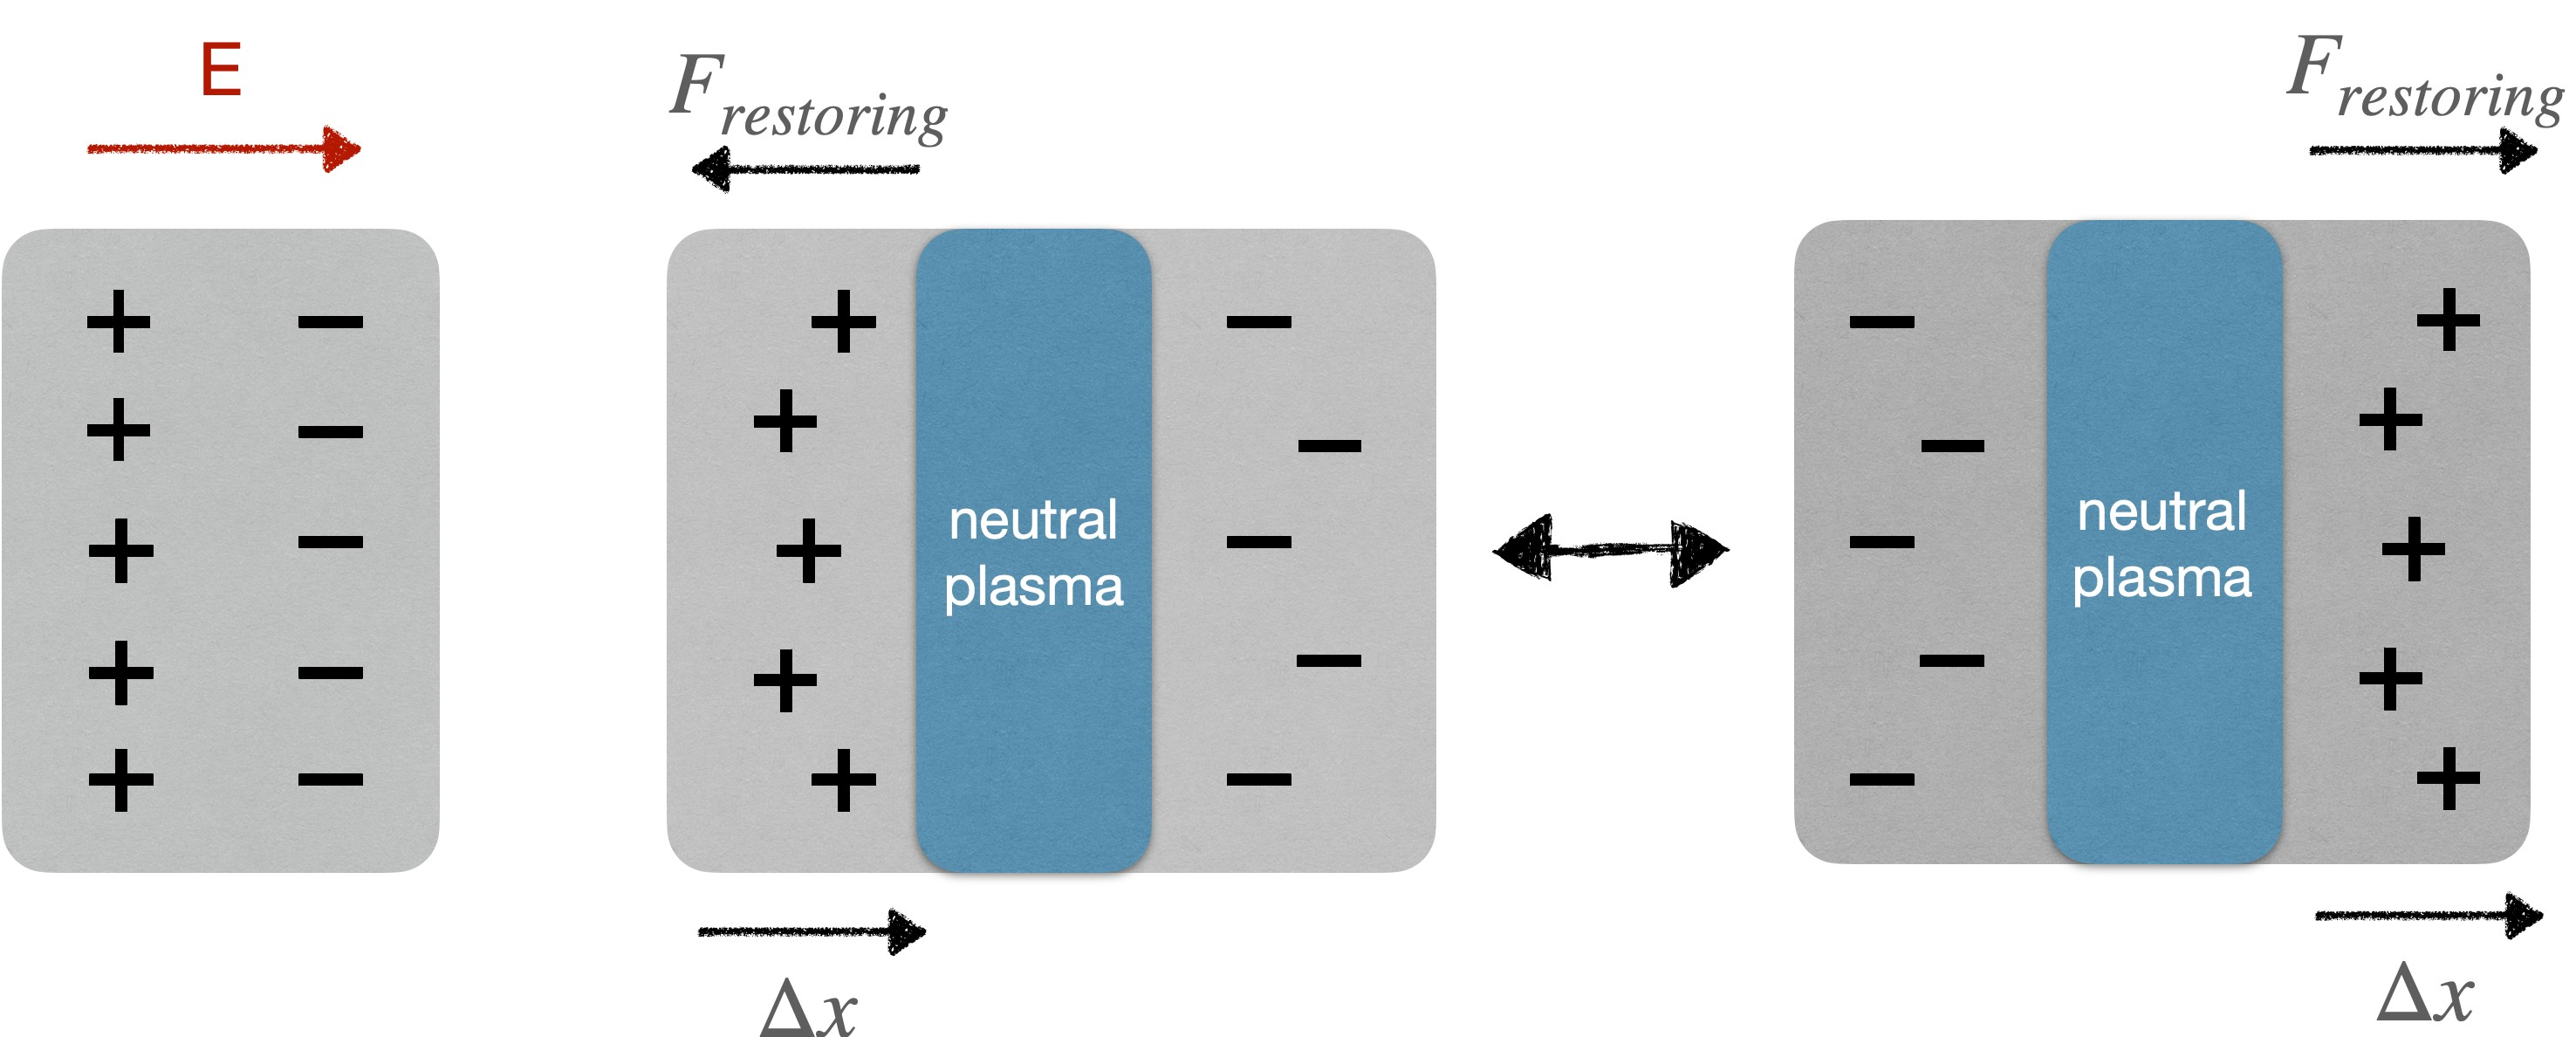
\includegraphics[scale = 0.1]{figures/plasma oscillator.jpeg}
  \caption{電子位移一小段距離 \(\Delta x\) 會產生 \(\sigma\) 的表面電荷,並且恢復力會導致特定頻率的振盪,具體頻率取決於電漿密度。}
  %{Displacement of electrons by a small distance \(\Delta x\) generates a surface charge of \(\sigma\), and the restoring force lead to oscillations at a specific frequency that depends on the plasma density.}
  \label{fig:plasma_oscillator}
\end{figure}

考慮一個靜止且分佈均勻的理想電漿,具有相同數量的電子與離子,電漿密度為\(n_{0}\) 。
這樣情況下的電動力學僅發生在極短的時間尺度,且由於離子的質量遠大於電子,發生運動的時間尺度比電子短上非常多,這樣時間尺度的差距下我們能夠將離子視為靜止。假設電子突然位移了\(\Delta x\) ,由於上述提及由庫倫力導致的恢復力,將會產生一個簡諧震盪運動。
恢復力造成了電漿的震盪,這也意味著透過恢復力能夠計算出\(\omega_{p}\)
想像一下,在理想化的電漿中(見圖 \ref{fig:plasma_oscillator}),電子和離子就像兩個重疊的電板。當電場將負電板向右驅動 \(\Delta x\) 時,它會將離子留在原地,而根據高斯定律,間隙中產生的電場 (E) 由下式給出
%Considering a stationary and uniformly distributed idealized plasma, with equal numbers of electrons and ions, with density \(n_{0}\). Electron dynamics occur on a very short time scale, and Since the mass of the ion is much larger than electrons, electron dynamics occur on a much shorter time scale than ions. If the interaction time is short enough, ions are considered as stationary during this time. Suppose the electron is suddenly displaced by the length \(\Delta x\), this creates a simple harmonic oscillator due to a restoring force generated between the stationary ion and the electron. The restoring force causes plasma oscillations, which means \(\omega_{p}\) can be calculated by the restoring force. Imagine that in idealized plasma (see Figure \ref{fig:plasma_oscillator}), electrons and ions are like two overlapping slabs. When the electric field drives the electrons to the right by \(\Delta x\), it leaves the ions to the left. By Gauss’s law, the electric field (E) developed in the gap is given by

\begin{align}
  \begin{split}
    E = \frac{\sigma}{\epsilon_{0}}
    \\
    = \frac{en_{e}}{\epsilon_{0}} \Delta x
  \end{split}
\end{align}

\(\sigma\) 表示面電荷密度,\(n_{e}\) 是電子密度,e則是電子的電量,\(\epsilon_{0}\)代表真空電容率,\(\Delta x\)是負電板的位移距離。
將電子拉回原位的力可以被寫成
%where σ is the charge density, ne is the electron density, e the charge of an electron, ε0 is the vacuum permittivity, and \(\Delta x\) the displacement of the electrons. The force pulling the electrons due to the displacement is
\begin{align}
  \begin{split}
    F = qE
    \\
    = \frac{e^{2}n_{e}}{\epsilon_{0}} \Delta x
  \end{split}
\end{align}

從牛頓第二定律可知,這式會變為二階線性常微分方程
%By Newton’s second law, this become a second order linear ordinary differential equation

\begin{align}
  \begin{split}
    m_{e}\frac{d^2}{dt^2}\Delta x = \frac{e^{2}n_{e}}{\epsilon_{0}} \Delta x
  \end{split}
\end{align}
其中 \(m_{e}\) 是電子的質量。 因此寫下振盪頻率:
%where me is the mass of an electron. This gives the frequency of the oscillation as:
\begin{align}
  \begin{split}
    \omega_{p} = \sqrt{\frac{e^{2}n_{e}}{m_{e}\epsilon_{0}}}
  \end{split}
\end{align}

\section{有質動力}%{Ponderomotive force}
電磁場對電漿運動具有影響力,當電漿中帶電粒子在雷射的電磁場影響下的運動,由於同時有電場(E)與磁場(B)的作用我們必須考慮勞倫茲力,其定義如下:
The electromagnetic field will affect the plasma. Charged particles move under the influence of the laser's electric E and magnetic B fields as it propagates through an underdense plasma, as defined by the Lorentz force:

\begin{align}
  \begin{split}
    \frac{dp}{dt} = q(E + \frac{v}{c}\times B)
  \end{split}
\end{align}

p,q,v分別代表粒子動量、電量以及速度,當電子速度遠小於光速v = c,此時勞倫茲力可以寫成
%where p is the particle momentum, q the particle charge, and v particle velocity.
%When the particle velocity is much less than the speed of light v = c. Then the Lorentz force can be written as

\begin{align}
  \begin{split}
    \frac{dp}{dt} = qE
  \end{split}
\end{align}

透過數學電磁場可以表示為\(E = ELsin(kz − \omega t)\hat{x} \),電子將以相同的頻率在極化方向上振盪。 該電子的歸一化動量為\(p_{x}/m_{e} c\)=\(v_{x}/c=a_{0}\) \(cos⁡(kz-\omega)\),其中\(a_{0}\)又稱為歸一化向量勢,其定義如下:
%\(E = ELsin(kz − \omega t)\hat{x} \) for the EM field. The electrons will oscillate in the polarization direction at the same frequency. The normalized momentum of this electron is \(p_{x}/m_{e} c\)=\(v_{x}/c=a_{0}\) \(cos⁡(kz-\omega)\) where \(a_{0}\) is the normalized vector potential defined as

\begin{align}
  \begin{split}
    a_{0} = \frac{eE_{0}}{m_{e}c\omega} = \sqrt{\frac{I[W cm^{-2}]\lambda_0[\mu m]}{1.37 \times 10^{18}}}
  \end{split}
\end{align}

當電場增加時,\(a_{0}\) 也會增加,被推動的電子非常接近光速。 此時,v × B 項不可忽略。當 \(a_{0}\) > 1 \cite{GG2011} 時,我們將使用相對論粒子討論電子的運動。通過對電磁場中電子的運動方程的雷射週期取時間平均值,可以得出以下方程
%When the electric field increases, \(a_{0}\) will also increase, and the pushed electrons are pretty close to the speed of light. At this time, the v × B term cannot be ignored. When \(a_{0}\) > 1 \cite{GG2011}, we will discuss the electron's motion using the relativistic particle.%; otherwise, we will use the non-relativistic regime.
%From taking a time average over the fast laser period of the equation of motion for an electron in an electromagnetic field one can derivethe following equation
\begin{align}
  \begin{split}
    \frac{d\langle p\rangle}{dt} = -\frac{e^{2}}{2m_e\omega_0^{2}}\nabla \langle E^{2} \rangle = -\frac{1}{2}m_ec^{2}\nabla \langle a^{2}\rangle = F_{p}
  \end{split}
\end{align}
假設相對論的質量增加可以忽略不計。 在雷射焦點處,從焦點中心有一個 \(a_{0}\)的梯度。 雷射脈衝中心的電子獲得更多的能量比遠離雷射焦點的電子還要來得多。 這也是一個電位梯度,電子將沿強度梯度從高強度區域推向低強度區域。
%Assume that the relativistic mass increase is negligible. At the laser focus, there is a gradient of a0 from the center of the focus. Electrons at the center of a laser pulse can gain more energy than electrons farther from the laser's focal point. This creates a potential gradient that pushes electrons from high-intensity regions to low-intensity regions along the intensity gradient.


\(F_p\) 稱為有質動力(ponderomotive force)。對於 \(a_0\) > 1,即高強度雷射的情況,出現了相對論效應,在計算有質動力時必須考慮相對論效應造成地迎向,通過 Quesnel 和 Mora 推導電子和電磁場的相對論運動,他們精確使用數學來描述聚焦的雷射脈衝。\cite{PhysRevE.58.3719} 相對論性的有質動力的以下式表達
%\(F_p\) is ponderomotive force.For \(a_0\) > 1, i.e. a high intensity laser. relativistic effects appear, and these must be considered when calculating ponderomotive forces,  A focused laser pulse is described through the precise calculations of the relativistic motion of an electron and electromagnetic fields carried out by Quesnel and Mora.\cite{PhysRevE.58.3719}They calculate the following expression for the relativistic ponderomotive force
\begin{align}
  \begin{split}
    \frac{d\langle p\rangle}{dt} = -\frac{1}{2}m_ec^{2}\frac{1}{\langle\gamma\rangle}\nabla \langle a^{2}\rangle
  \end{split}
\end{align}
其中 \(\langle\gamma\rangle\) 是快速震盪的平均\(\gamma\) 。 這意味著由於在雷射電場的振動(quiver motion)中獲得的相對論質量增加,有質動力會減小。
%where \(\langle\gamma\rangle\)is the averaged gamma over a fast oscillation. It means that due to the increase in the relativistic mass obtained in the quiver motion, the ponderomotive force decreases.
\section{電漿中的非線性效應}
我們已經看到,考慮到顫動運動引起的平均質量增加,可以推導出有質動力的相對論表達式。有質動力將導致實際的電子位移,從而導致電漿密度的擾動,以及由於折射率梯度引起的雷射局部頻率的擾動。藉此我們又可以分別討論縱向以及橫向效應的影響。\cite{doi:10.1063/1.1692942}
折射率的橫向變化將使雷射的波前向更高的折射率彎曲。在雷射脈衝中,中心的強度更高,這導致更高的相對論質量增益,因此中心的折射率更高。這種圍繞光束中心旋轉對稱的折射率會導致類似於聚焦透鏡的波前曲率,因此通常被稱為「相對論自聚焦(relativistic self-focusing)」。此外,有質動力將電子推離中心,導致中心的密度較低,因此中心的折射率也較高。 對於相對論自聚焦的情況,可以推導出一個閾值,在該閾值處雷射繞射與傳播取得平衡,因此稱為「相對論性自導(relativistic self-guiding)」。

縱向方面,考慮到電子被雷射向後排開,脈衝末端的密度低於前面的密度。這意味著前面移動的速度比後面慢,因此脈衝將被壓縮。對於比 \(c/\omega_p\) 還長的脈衝,連續的壓縮和拉伸將導致雷射脈衝分裂成幾個由 \(c/\omega_p\) 分隔的子束\cite{doi:10.1063/1.1692942},這個過程又稱為「自調製(self-modulation)」。
\section{雷射電漿波加速器的產生}
在本節中,我們將介紹強激光脈衝與等離子體相互作用的物理學,並通過開發非線性一維低溫流體模型來計算產生的尾流場。該模型忽略了激光場和等離子體特性的橫向變化,這意味著該模型僅在激光脈衝軸附近有效。然而,它可以幫助我們理解尾場的某些基本屬性。在我們的一維模型中,假設等離子體離子是不動的,因為它們的質量要大得多,而且激光脈衝的傳播速度很快。等離子體將再次被視為零溫度的電子流體。這個假設意味著粒子最初是靜止的,從而使我們可以忽略由於電子熱運動引起的影響。將導出描述一維激光尾場的靜電勢非線性微分方程。
當高強度的雷射脈衝撞擊電漿時,電子將受到有質動力,將它們推到雷射脈衝前面和側面。由於離子比電子重得多,位移的電子和靜止離子會引起電荷分離,從而導致等離子體振盪跟隨脈衝。這些被稱為尾場振盪,可以是線性的或非線性的,具體取決於驅動雷射脈衝的強度。
當雷射以群速度 \(v_p \approx \sqrt{1 - \frac{\omega_p^2}{\omega_0^2}}\) 傳播時,雷射將持續將電子推開。
儘管每個振盪區域在低溫電漿中本質上是獨立的,但由於雷射驅動著電漿波,電漿波相速度應等於為雷射的群速度。這意味著電漿波也有一個波長可由\(\lambda_{p} = \frac{2\pi v_g}{\omega_p}\)關係得知。
當電磁場開始從雷射傳播方向橫向振蕩,該條件在雷射脈衝後面和雷射光軸上產生一個從四分之一電漿波長到一半電漿波長的區域,會持續恆地出現一個電場
利用高斯定律對一維電漿波在線性求解 \cite{kta2008} \cite{gibbon2005short} ,
\(E = E_{max}Lsin[\omega_{p} (z / v_{p} - t)]\) 和 \(v_p \approx c\),
假設所有電子都以波數 \(k_p = \omega_p/c \) 振盪,得出電漿中可達到的場強度估計值:
\begin{align}
  \begin{split}
    \frac{E_{max}}{E_0} = \frac{a_{0}^2}{\sqrt{1+a_{0}^2}}
  \end{split}
\end{align}
%Solving  Gauss’s  law  in  a  1D  linear  case \cite{kta2008} \cite{gibbon2005short}  for  a  plasma  wave,\(E = E_{max}Lsin[\omega_{p} (z / v_{p} - t)]\), and \(v_p \approx c\), under the assumptionthat all electrons oscillate with the wave number\(k_p = \omega_p/c \), yieldsan estimate of field strengths attainable in plasmas:
顯示了驅動脈衝(紅色)兩個不同 a0 值的數值求解的電漿電動勢、電場和密度(海軍線)。圖 \ref{fig:linearwakefield}中對於低 a0 驅動脈衝,正弦尾流跟隨雷射脈衝。圖 \ref{fig:wakefield}一旦 a0 > 1,尾流開始變得非線性,電子密度開始出現尖峰,電場呈鋸齒狀。震盪的波長增加了,這是由於相對論質量隨著尾流中粒子的速度接近光速(β → 1)而增加。
\begin{figure}[h]
  \centering
  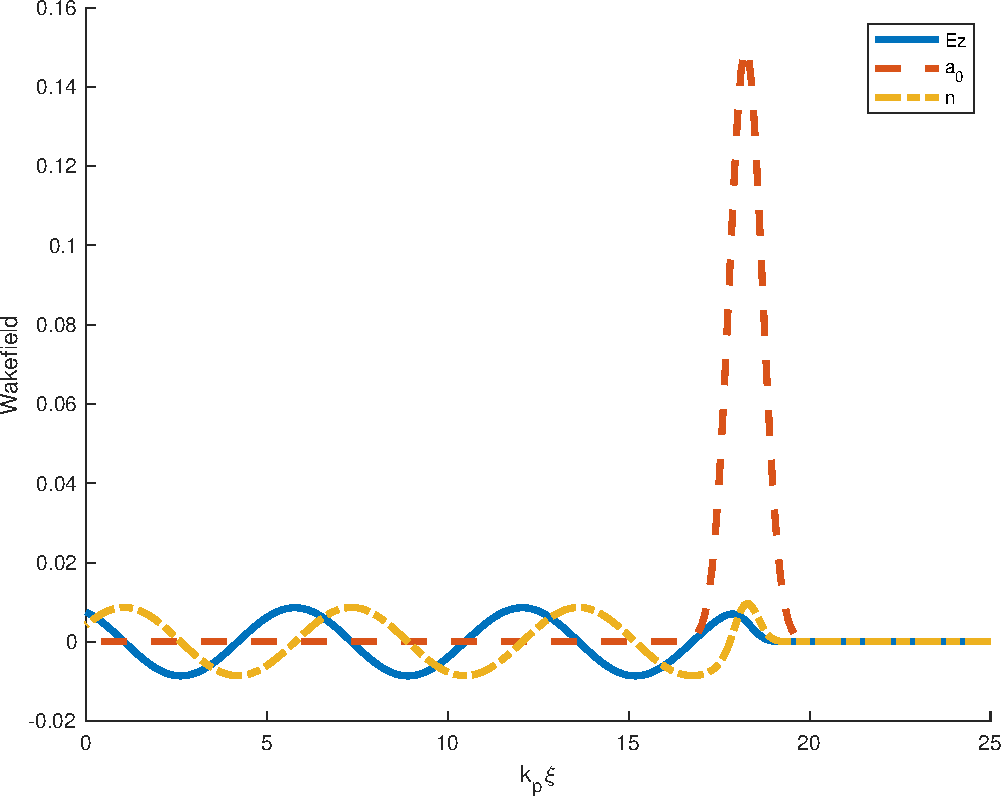
\includegraphics[scale = 0.6]{figures/linearwakefield.pdf}
  \caption{}
  \label{fig:linearwakefield}
\end{figure}
\begin{figure}[]
  \centering
  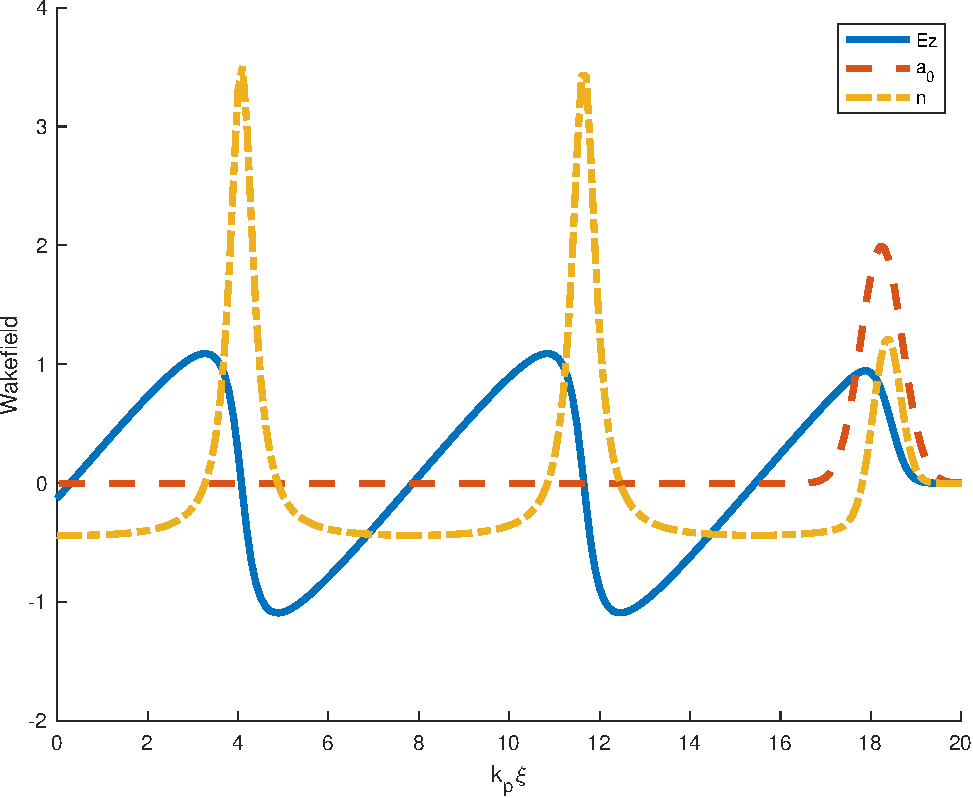
\includegraphics[scale = 0.6]{figures/wakefield.pdf}
  \caption{}
  \label{fig:wakefield}
\end{figure}

\section{泡泡結構與相位空間}%{Bubble regime and phase space}
有助於理解注入的一個重要概念是由粒子脈衝跨越的相空間及其在位(potential)中的位置。在與時間無關的拋物線位中,可以從相空間圖的任意位置開始,也就是初始粒子位置和動量,並求解運動方程,將獲得閉合軌道相空間軌跡。
這表示振盪運動,因為拋物線勢中的運動方程會產生諧振震盪。這個粒子將被困在位能中,軌跡代表位能和動能的總和。對於時間與無關的位能和線性運動,這些不同能量的軌跡永遠不會交叉。考慮像雷射脈衝產生的尾流這樣的周期性有限位,那麼將存在相空間軌跡,其中粒子可以穿位能井並逃逸到無窮大。在 LWFA 的背景下,這些軌道代表形成尾流的背景電漿電子,因此被稱為流體軌跡。在被困軌跡和流體軌跡之間是一條特殊的軌跡,將這兩個區域分開,稱為分界線(separatrix)。上述相位移動極限由縱向相空間中給定相空間軌跡的最高脈沖值表示。通常加速器長度被限制為一個相移長度,但如果雷射隨著傳播不會消耗能量或散射,也可以加速超過一個半相移長度並獲得相同的結果。粒子的全相空間必然是 6D 相空間,並且在 LWFA 中,粒子也會在橫向上被捕獲,經歷電子感應加速器振盪。可以證明 [42-44] 橫向振盪電子感應加速器頻率 ωB 是針對縱向加速度的相對論質量增益校正的電漿頻率。
\section{注入方式}
通過電漿傳播的高強度雷射脈衝形成了尾流,但這種結構的形成本身並不會產生高能電子。為了產生高能電子,電子必須與形成波的電子分離,並注入電漿波的加速區。圖 顯示了這一點:電子必須在分界線內才能從尾流中獲得能量。 從哈密頓量分析中我們看到,電子必須具有一定的最小初始速度,並且注入必須發生在一定的相位範圍內(即時間和位置的組合),然後電子才能被困在尾流的加速階段。 此外,注入的細節,例如注入電子束的初始能量和動量分佈或持續時間,將強烈決定加速電子束的特性,如:持續時間、能量擴散和發射率,我們也將之合稱為加速後的電子品質。 因此,在雷射尾場加速器中注入電子是一個關鍵部分,並且正在受到各種研究。

接下來的段落概述幾種電子注入尾流的方法,更先進的機制可以產生更穩定的電子束,這對於實驗應用很有幫助。而注入方式主要分為兩種,自發注入及激發注入。

 \subsection{自注入}
自發注入這種方式,是利用捕獲來自背景電漿的一些電子並在尾場的適當相位中加速,從而產生飛秒等級的相對論性電子束。
內部注入的一個例子是最近展示的“氣泡(Bubble)”注入方法\cite{Wang_2018}。 這種方法提供的電子束團具有 185 MeV 量級的能量和低於10\%的相對能量散佈。 然而,這種方法仍然存在較差的穩定性。
近期Kosta Oubrerie也有透過使用長達15mm的電漿通道來增加加速長度,產生了單能的 1.5 GeV 電子束,其能量分佈為 3.7\%。\cite{cite-key}
\subsection{衝擊波注入}
電漿密度轉變也可用於誘導 LWFA 中的注入。 2010 年,K. Schmid 等人在\cite{PhysRevSTAB.13.091301} 中首次展示了以急劇的密度差區域注入電子。雷射脈衝進入高等離子體密度區域,然後過渡到低密度區域。發生注入是因為電漿波長與 \(\lambda_p \propto \sqrt{n}\) 成正比。因此,電漿波的結構在電漿密度的過渡點突然發生了變化。突然的轉變導致來自高密度尾流振蕩的一些電子最終進入低密度等離子體波的相空間的捕獲區域。為了使這種注入方法起作用,密度轉變必須是電漿波長的數量級 \cite{Brantov2008},對於 \(10^{18}\) 到 \(10^{18}\ cm^{-3}\) 的電漿密度,其約為 10μm。這些剖面是通過使用超音速噴流和障礙物(刀片)\cite{Brantov2008} 結合氣體射流和毛細管達成的。
\subsection{電子加載}
隨著電荷被注入尾流中,注入的電荷也將有助於尾流的形成。尾流加速階段的電子通常會降低有效加速場強度。 Tzoufraset 等人在理論上對此進行了研究。 [47],其中得出的結論是,在一定長度的電子束中,加速場的降低程度不同,具體取決於電荷分佈。通常,這會導致初始單能電子束的能量擴散增加。 Rechatinet 人。 \cite{Rechatin2009}已經證明了這種效應的實驗觀察,使用碰撞脈衝注入。通過調整反向傳播脈衝的脈衝能量,他們能夠在其他不變的加速條件下調整注入的電荷量。他們觀察到當電荷從 1pC 變化到 20pC 時,電子能量減少了 15\%。他們還觀察到能量擴散的比例增加。碰撞脈衝注入的方法預計會在很短的距離內發生,但在高電荷的情況下,在 170 MeV 的峰值電子能量處觀察到 25\% 的能量擴散。
\section{Betatron 輻射}
在電漿波的氣泡結構,尾流中包含有在雷射傳播方向上加速的電場,以及在橫向方向上的聚焦場。 這意味著注入偏離中心軸注入的電子將在尾場中振盪。電子的這種固有的橫向運動被稱為電子感應加速器振盪,並將產生 X 射線輻射 (10-100keV)
\cite{PhysRevLett.93} ,由於其微米級的源尺寸和高空間相干性,非常適合發展相襯顯微技術[79-82]。
 這種輻射與同步輻射非常相似,但由於電漿波長明顯更短,尾流產生的震盪器的尺寸又比聚頻磁鐵小數個數量級,並且需要能量較低的電子束(MeV 而不是 GeV)。 聚頻磁鐵/增頻磁鐵是一種具有周期性磁場結構的裝置,可使電子通過時產生振盪,用於同步加速器和自由電子激光器。
\section{LWFA 實驗設計}
 實驗示意圖如圖,我們使用衝擊波注入來產生單能電子束,實驗室內所使用雷射光源是利用啾頻脈衝放大器(chirped pulse
amplification,CPA)雷射系統\cite{Maine137}。雷射在最後輸出單發能量為3.3 J, 中心波長808 nm,脈衝寬度33 fs(1 fs = \(10^{-15}\) sec),重複頻率為2 Hz。把雷射光聚焦到實驗用的靶材上可產生超過\(10^{19} W/cm^{2}\) 的尖峰強度。利用離軸拋物面鏡(OAP)將雷射聚焦在一個3mm噴嘴上方,而噴嘴上方則有銳利的刀口遮蔽超音速氣體噴嘴的前端,如此便可產生衝擊波,以製造一個電漿密度陡峭的斜坡,使電子能夠被注入。
推測電漿通道的工作範圍大約為3500\(\mu m\),密度斜坡長度約為10\(\mu m\) 。
此外我們將刀口裝置於一個旋轉平移台上,想藉由旋轉製造密度斜坡橫向的角度變化,這也是後續模擬的一大重點。
電漿通道後方我們利用一個偶極磁鐵產生約為1.2T的磁場作為光譜儀分析電子能量。

\section{PIC 模擬}
在構建實驗之前通過模擬研究電漿尾場加速有兩個主要原因。儘管模擬的會花費的時間遠大於實驗數據的產出,但依賴高性能計算機的支援 (HPC),模擬能夠清楚記錄電漿波短時間內的細節變化,讓我們有機會探究電漿波的細部物理現象。模擬第二個優勢在於參數可以根據各式需求自由更動,但受限於計算機性能的限制,而傳統的加速器或雷射器的參數通常只能在相對較小的範圍內變化,這麼一來便可省下龐大的資源集中研究某個參數範圍內的物理現象。
即便模擬具有上述優勢,但實驗仍然是必要的。模擬很難充分考慮現實世界的因素,例如啟動參數的變化和缺陷以及外部干擾。模擬還必須對所研究現象的長度和時間尺度做出假設,並選擇時間步長和空間分辨率等參數以解決這些問題。由於模擬可能出現數值錯誤或不符合物理的現象,或實驗可能會展現出預期之外的行為。
因此,模擬和實驗都是開發粒子加速器新技術的有用和必要的工具:模擬提供了一種方便的方法來以低成本和時間開發新概念,而後透過實驗在現實世界中驗證模擬結果也是不可或缺的。

電漿由一組在電磁場中移動的帶電粒子(電子和離子)組成。場由帶電粒子的分佈和速度決定,而粒子的運動由場和初始條件決定。電漿尾場加速中在乎電漿具有厘米的典型尺寸和 \(10^{20} m^{-3}\)  的密度。
對於體積為 \(1cm^3 = 10^{-6} m^{3}\) 在此密度下的電漿,總粒子數約為 \(10^{14}\)。模擬中的每個粒子都必須有許多與之相關的位置和速度分量,每個分量通常由一個 32 位雙精度浮點數表示,每個粒子需要數百位的暫存。
因此,對每個真實粒子進行建模的總內存需求至少為 \(10^{15}\)位元。鑑於計算機內存容量以千兆bytes為單位,即大約 \(10^{9}\)bytes,對如此大量的粒子進行建模遠遠超出了當前計算機。
即使這樣的計算機可用,仍然非常需要一種更有效的方法來執行這些模擬。
可以將粒子建模為流體或大粒子或超粒子,其中大量真實粒子由單個大粒子表示,該大粒子攜帶其所代表的粒子的組合電荷和質量。與粒子模型相比,流體模型受到限制,因為它不允許在單個區域中存在碰撞或粒子速度分佈。在粒子單元模擬中,粒子位置和速度(相空間坐標)是連續值,而場是在模擬網格上計算的。
然後使用有限差分法求解麥克斯韋方程和粒子的運動方程,因此模擬在空間和時間上是離散的。離散化對於在具有有限內存的計算機上模擬等離子體是必要的。由於場的分辨率受網格間距的限制,大粒子模型可以是有效的,因為由相同大粒子表示的真實粒子將看到相似的場並因此一起移動。
PIC模擬是透過有限差分法進行計算,通過用有限差分代替導數來近似微分方程的解。 如果導數是關於時間的,則有限差分是時間步長。 Yee 開發了一種有限差分時域算法,用於求解各向同性介質中的馬克思威方程組。 在粒子模擬中,不同於純電磁模擬,一旦計算了電場和磁場,粒子就會被推動。 根據作用在它們上的力更新粒子位置,新的粒子位置用於計算電荷密度和電流密度,然後再次用於計算場。 該算法的說明如圖所示。
IC 模擬中的粒子推動通常使用跳躍式方法,其中粒子位置和速度以交替的半時間步長計算,因此不會同時進行紀錄。
%Simulation is a useful tool to study new techniques of laser wakefield acceleration, which provides a convenient method to develop new concepts at low cost and time. Simulation parameters can be more flexibly adjusted than experiments. Despite the advantages of simulation, it still cannot fully represent all situations in the real world. The simulation must have a reasonable assumption of length and time scale in different phenomena and choose parameters such as appropriate time step size and spatial resolution to address these issues.

\section{PIC模擬設定}
我們使用VORPAL中二維模擬研究了使用密度剖面注入方法的 LWFA 的性能。 雷射脈衝寬度的半峰全寬 (FWHM) 為 33 fs,雷射波長為 810 nm,雷射強度參數 \(a_0 = 3.2 ~ 6.3\)。 電漿密度 \(n_e\) 在 \(10^{18}~10^{19} cm^{-3}\) 範圍內變化,用於研究單能電子束。 相對論光導的雷射功率 P 與臨界功率 \(P_c\) 之比約為 1.4 ~ 4.2(對應於 \(n_e = 10^{18}~10^{19} cm^{-3}\)。 因此雷射脈衝可以在沒有外部引導的情況下通過 3.5 mm 的氣體射流傳播。 這
模擬框中的網格點數為 \(N_x, N_y) = (4096, 512)\),網格大小 \(\Delta x =\lambda/32 , \Delta y = 4 \Delta x\),分別在 x 和 y 方向。 時間步長由 Courant 條件的 0.99 倍決定。

% !TeX root = ../main.tex

\chapter{利用衝擊波注入達到單能電子束}%{Achieve monoenergetic electron beam with shock front injection}

雷射尾場加速器有著相當廣泛的應用,其中之一是用於 FEL 的加速電子源。 然而,用於 FEL 的電子源具有非常嚴格的質量要求,為了製作可投入聚頻磁鐵使用的電子源。 找出可以產生單能電子的參數及方法是必要的,我們通過參數掃描和優化單能電子譜來觀察各項參數對於衝擊波注入影響及趨勢。 然後討論這些參數如何在物理上影響我們加速電子的品質。
% Laser wakefield accelerators are used in a wide range of applications, one of which is an accelerated electron source for the FEL. However, an electron source for the FEL has quite stringent quality requirements to produce an electron source that can be put into the undulator. It is necessary to find out the parameters that can produce monoenergetic electrons, and we find the trend through the parameters scanning and optimizing the monoenergetic electron spectrum. And then discuss how these parameters physically affect the quality of our accelerated electrons.
在 NCU 100TW 雷射系統中,對於焦點 \(w_{0}\) 低於 \(10\mu m\) \(a_{0} \simeq \) 4.3,這比其他研究要大很多,所以 \cite{Rechatin_2010} 當注入過多的電子時會抵消氣泡區內的加速場,導致部分電子無法加速,電子能散也因此變大。 本章節展示了不同能量雷射在電漿中的演變,以及雷射在高密度電漿區域的非線性效應對注入的影響。
% In NCU 100TW laser system, for the focus spot \(w_{0}\) is lower than \(10\mu m\) \(a_{0} \simeq \) 4.3, which is quite large than other study, so that the ponderomotive force will cause excessive electron injection.\cite{Rechatin_2010} Too many electrons will offset the acceleration field inside the bubble regime, causing part of electrons to fail to accelerate and disperse the electron spectrum. This chapter demonstrates the evolution of lasers of different energies in the plasma and the impact of the nonlinear effects of lasers in the high-density plasma region on injection.
\section{電子加載優化}%{Optimization of beam loading}

% In order to profit from the beam loading effect to optimize the energy spread at the exit of the plasma channel, it is desirable to have control charge to avoid overload.
\subsection{\(a_{0}\) 對氣泡結構的影響}%{Influence of \(a_{0}\) on bubble structure}

\subsection{通過加載優化減少能散}

\subsection{優化自聚焦}%{Optimize self-focusing}


\section{Discussion}

% !TeX root = ../main.tex

\chapter{Injection mechanism of tail wave injection}
在上面章節中我們發現,雖然都是透過衝擊波產生的密度斜坡進行LWFA的注入,顯然這項結果與過去多數的研究結果並不相似。
我也成功還原出比較接近於多數研究的模擬,並且從各項電子品質進行分析與比較。
分析出此種注入的機制以及其優點與缺點。
% In the above section, we found that although the LWFA injection was carried out through the density slope generated by the shock wave, it is obvious that this result is not similar to that of most previous studies.I have also successfully reproduced simulations that are close to most studies, and analyzed and compared various electronic qualities.The mechanism of this injection and its advantages and disadvantages are analyzed.
\section{尾波注入和加載注入的電子特性比較}%{Comparison of electron injection characteristics between tail wave injection and beamloading injection}



\section{Differences in tilted shock-front performance}


\section{Discussion}


% 參考文獻
% References
\refmatter
% \bibliographystyle{abbrv}
% \bibliography{back/references.bib}
% \printbibliography
% 附錄
% Appendices
% % !TeX root = ../main.tex

\appendix{A}{Introduction}
\section{Introduction}
\section{Further Introduction}

% % !TeX root = ../main.tex

\appendix{B}{Introduction}
\section{Introduction}
\section{Further Introduction}


\end{document}
